\documentclass[a4paper,justified]{tufte-handout}

%opening
\title{Receiver Operating Characteristic (ROC) Curves}
\author{}

\usepackage{graphicx} % allow embedded images
	\setkeys{Gin}{width=\linewidth,totalheight=\textheight,keepaspectratio}
	\graphicspath{{graphics/}} % set of paths to search for images
\usepackage{amsmath}  % extended mathematics
\usepackage{booktabs} % book-quality tables
\usepackage{units}    % non-stacked fractions and better unit spacing
%\usepackage{multicol} % multiple column layout facilities
\usepackage{lipsum}   % filler text
\usepackage{fancyvrb} % extended verbatim environments
	\fvset{fontsize=\normalsize}% default font size for fancy-verbatim environments
\usepackage{booktabs}
\usepackage{multirow}
% Standardize command font styles and environments
\newcommand{\doccmd}[1]{\texttt{\textbackslash#1}}% command name -- adds backslash automatically
\newcommand{\docopt}[1]{\ensuremath{\langle}\textrm{\textit{#1}}\ensuremath{\rangle}}% optional command argument
\newcommand{\docarg}[1]{\textrm{\textit{#1}}}% (required) command argument
\newcommand{\docenv}[1]{\textsf{#1}}% environment name
\newcommand{\docpkg}[1]{\texttt{#1}}% package name
\newcommand{\doccls}[1]{\texttt{#1}}% document class name
\newcommand{\docclsopt}[1]{\texttt{#1}}% document class option name
\newenvironment{docspec}{\begin{quote}\noindent}{\end{quote}}% command specification environment

\begin{document}
\maketitle

\begin{fullwidth}
\noindent A Receiver Operating Characteristic (ROC) curve is a graphical plot which presents the performance of a binary classifier when the discrimination cut-off, or threshold, is varied. The ROC curves and associated analysis, such as area under the curve, comparing multiple ROC curves and finding an optimal threshold, have proved very useful analysis tools in many fields of research such as medical diagnosis and disease management. They have been found to be a more appropriate technique for evaluating diagnostic and predictive accuracy.

\vspace{3mm}
\noindent Essentially for creating and plotting the ROC curve one needs to compute the true positive rate (TPR) and the false positive rate (FPR) at various threshold settings and plot them in a dimensional space. In machine learning the TPR is referred to as the sensitivity or recall which measures the proportion of actual positives that are correctly classified. The true negative rate (TNR), or specificity, measures the proportion of actual negatives that are correctly identified as such. These measures can be easily summarised in Table 1 below.

\begin{table*}[h]
	\begin{tabular}{@{}llccll@{}}
		\toprule
		\multicolumn{2}{l|}{}                                                                                                                               & \multicolumn{2}{c|}{\textit{True Class}}                                                                                                   & \multicolumn{2}{l}{}                                      \\ \midrule
		\multicolumn{1}{l|}{\multirow{2}{*}{\textit{\begin{tabular}[c]{@{}l@{}}Predicted \\ Class\end{tabular}}}} & \multicolumn{1}{l|}{Yes / 1 / Positive} & True Positives                                            & \multicolumn{1}{c|}{\begin{tabular}[c]{@{}c@{}}False\\ Positives\end{tabular}} & \multicolumn{1}{l|}{TPR = TP / P} & Sensitivity = TPR     \\
		\multicolumn{1}{l|}{}                                                                                     & \multicolumn{1}{l|}{No / 0 / Negative}  & \begin{tabular}[c]{@{}c@{}}False\\ Negatives\end{tabular} & \multicolumn{1}{c|}{True Negatives}                                            & \multicolumn{1}{l|}{FPR = FP / N} & Specificity = 1 - FPR \\ \midrule
		\multicolumn{2}{c}{\textit{Totals}}                                                                                                                 & \textbf{P}                                                & \textbf{N}                                                                     & \multicolumn{2}{l}{}                                      \\ \bottomrule
		\caption{Sensitivity and Specificity}
		\label{tab:normaltab}
	\end{tabular}
\end{table*}

\vspace{3mm}
\noindent ROC curves are widely used in medical applications. Consider a diagnostic test that seeks to determine whether a person has a certain disease. This is a two-class prediction problem in which the outcome is labelled either positive or negative. In this case there are four possible outcomes from the discrete classifier: true positive or true negative if the outcome matches the actual class, false positive if the person is incorrectly classified as sick, and false negative if the person is incorrectly classified as healthy. If the test is extended to a larger sample then given a classifier and a set of instances, a 2x2 contingency table, or confusion matrix, can be constructed representing the dispositions of the set of instances. Extending the test further to five classifiers, A to E, an ROC curve can be plotted, figure 1 (adopted from \citep{fawcett2006introroc}), with TPR on the y-axis and FPR (or 1 – specificity) on x-axis, which defines our ROC space depicting the relative trade-offs between true positives (benefits) and false positives (costs). 
\end{fullwidth}

\vspace{3mm}
\noindent The diagonal line from (0,0) to (1,1) characterises a test that cannot distinguish between diseased and non-diseased states, that is, a random guess. This line often serves as a benchmark for judging how well (or bad) a test performs.

\begin{marginfigure}[1.5cm]
	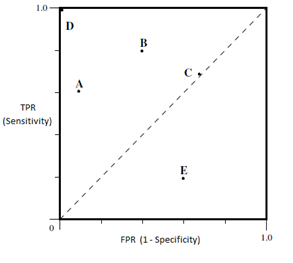
\includegraphics[width=\linewidth]{roc_curves/Figure1.png}
	\caption{Basic ROC plot with five classifiers.}
\end{marginfigure}

\vspace{3mm}
\noindent The best possible prediction method would yield a point in the upper left corner of the ROC space representing 100\% sensitivity and 100\% specificity, i.e. a perfect classifier. On the other hand, a random guess would outcome a point along or close to the diagonal line. Classifiers A and B yield good classification results whilst points below the line represent bad results (worse than random). The ROC plot allows us to compare classifiers and choose the one that is closest to (0,1) and furthest from TPR equals FPR (the diagonal line).

\begin{fullwidth}
\vspace{3mm}
\noindent Consider now that the blood protein levels in diseased people and healthy people are normally distributed. A medical test might measure the level of a certain protein in a blood sample and classify any number above a certain threshold as indicating disease. Thus given a threshold parameter $p$, the instance is labelled positive if the continuous random variable $X$ is greater than $p$ and negative otherwise. As shown in figure 2 (left), choosing a high threshold produces a low likelihood of a false positive (while increasing the specificity) and a high likelihood of a false negative result (while decreasing sensitivity). Choosing a low threshold results in the opposite effect. Thus a different threshold would result in a different sensitivity and specificity pair. By repeating the experiment with adjusted thresholds different values for FPR and TPR are obtained leading to different positioning in the ROC space. The classifier that is able to increase the rate of detection while keeping the false alarm rate low is considered a good classifier. Figure 2 (right) shows the ROC curves with different thresholds. As the ROC curve gets closer to the top left hand of the graph the more optimal the threshold and the better the ability to discriminate between the classes.
\end{fullwidth}

\begin{figure}
	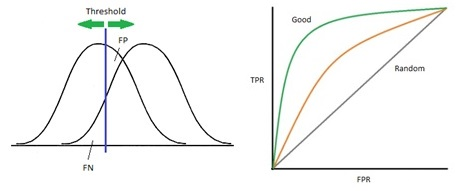
\includegraphics[width=\linewidth]{roc_curves/Figure2.png}
	\caption{Left: Distributions of results for a hypothetical continuous diagnostic test. Right: ROC curves with different thresholds.}
	\label{fig:fullfig}
\end{figure}

\begin{fullwidth}
\noindent The most common condition for choosing the optimal parameterisation is to maximise the area under the curve, AUC for short. The AUC, defined as $\int_{0}^{1} ROC(t) dt$ is a widely used measure of performance of supervised classification rules. It is a measure of the usefulness, or rather the discriminatory ability, of a test in general where the greater the area the more discriminative the test is in a given situation. A model or test with perfect discriminatory ability will have an AUC of, or very close to, 1.0, while a model unable to distinguish between individuals with or without the chosen outcome will have an AUC value of 0.5.  No realistic classifier should have an AUC less than 0.5. 

\end{fullwidth}

\begin{marginfigure}[6.0cm]
	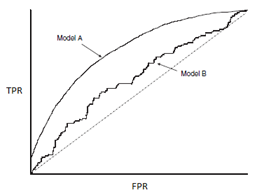
\includegraphics[width=\linewidth]{roc_curves/Figure3.png}
	\caption{A comparison of two AUC curves.}
\end{marginfigure}

\vspace{3mm}
\noindent However, the true value of AUC comes when comparing two or more models or tests by reducing the ROC to a single scalar value representing the expected performance of the models. Figure 3 (adopted from \citep{linden2006diagpreddismgmt}) provides a comparison between two predictive models. Model A is both statistically and visually better at identifying individuals with and without the outcome than Model B since the AUC is bigger. Therefore, if a choice was to be made between selecting one of the models, Model A would be the choice.

\vspace{3mm}
\noindent AUC is a desirable measure because (1) it is scale-invariant: it measures how well predictions are ranked rather than their absolute values; (2) AUC is classification-threshold-invariant: it measures the quality of the model’s predictions irrespective of the classification threshold chosen.

\begin{fullwidth}

\vspace{3mm}
\noindent ROC curves are typically used in binary classification problems but what about multi-class problems? In order to extend ROC analysis to multi-class or multi-label classification, it is necessary to binarise the output. A multi-class problem introduces the issue of combining pairwise discriminability values. One approach introduced by Provost and Domingos \citep{provost2003treeind} was to generate each class reference ROC curve, in turn measure the AUC, then assuming the AUCs are weighted by the reference class’s prevalence in the data. More precisely, $AUC_{total} = \sum AUC(c_{i}).p(c_{i})$ where $c_{i}\in C$ the set of all thresholds, and $p$ is the probability of class membership.
The disadvantage with this method is that the class reference ROC is sensitive to class distributions and error costs, so is the formulation of $AUC_{total}$.

\vspace{3mm}
\noindent To overcome this problem Hand and Till \citep{hand2001aucmulticlass} suggested a derivation that is based on the fact that the classifier will rank a randomly chosen positive instance higher than a randomly chosen negative instance. From this probabilistic form, they derived a formulation that measures the unweighted pairwise discriminability of classes. While this formulation is well justified and is insensitive to changes in the class distribution, they found no easy way to visualise the surface whose area is being calculated.

\vspace{3mm}
\noindent Thanks to its close relationship with yet another widespread Wilcoxon statistic \citep{hanley1982useauc}, AUC methods for AUC-based analyses are well developed and widely used. However one of the major practical drawbacks of the AUC as an index of diagnostic performance is that it summarises the entire ROC curve including the regions that frequently are not relevant to practical applications, such as regions with low level of specificity, according to Ma et al. 2013 \citep{ma2013paucdiagperf}. To alleviate this deficiency while benefiting from some of the advantageous properties of the area under the ROC curve, one can use a partial area under the curve (pAUC for short), which summarizes a portion of the curve over the prespecified range of interest. A number of approaches have been developed for pAUC-based analysis \citep{dodd2003pauc,he2010nonparagenomic,mcclish1989paucanal,zhang2002nonparpaucapp}. However, Ma et al. argue that the same features that increase the practical relevance of the pAUC introduce some difficulty to resolve issues related to arbitrariness of specifying the range of interest. 

\end{fullwidth}

\begin{marginfigure}[7.0cm]
	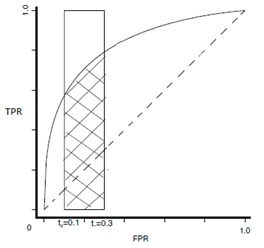
\includegraphics[width=\linewidth]{roc_curves/Figure4.png}
	\caption{Illustration of an ROC curve and its partial AUC with $t_{0}$ = 0.1 and $t_{1}$ = 0.3.}
\end{marginfigure}

\vspace{3mm}
\noindent Dodd and Pepe \citep{dodd2003pauc} claim that in population screening, in order to avoid high monetary costs the region of the curve corresponding to low false-positive rates is of primary interest. In diagnostic testing it is critical to maintain a high TPR in order not to miss detecting diseased subjects. They go on to consider a summary index for the ROC curve restricted to a clinically relevant range of false-positive rates.

\vspace{3mm}
\noindent Essentially the partial AUC is simply the area under the ROC curve between $t_{0}$ and $t_{1}$ (Figure 4) where the interval ($t_{0},t_{1}$) denotes the false-positive rates of interest. The partial AUC is expressed as

\[AUC(t_{0},t_{1}) = \int_{t_{0}}^{t_{1}} ROC(t)  dt\]

\begin{fullwidth}

\noindent Selecting the interval is an important practical issue but it is beyond the scope of this essay to delve further.

\vspace{3mm}
\noindent ROC curves have been used by numerous authors to evaluate models and scoring systems developed for pest risk assessment \citep{copp2009screening,heidy2010minfneginvspec}. They conclude that, in comparison with other models, the strength of the ROC analysis is that it thoroughly investigates test accuracy across a range of scores, and that it allows for visual examination of scores on one curve or a comparison of two or more curves using a similar metric. This allows analysts to easily determine which decision threshold is most preferred, based on the desired trade-off between sensitivity and specificity, or to establish which model has the best accuracy based on the largest AUC \citep{linden2006diagpreddismgmt}. In a later paper Makowski and Mittinty \citep{makowski2010scorsysinvpests} present a procedure based on Monte Carlo simulations and ROC analysis to assess and compare scoring systems for invasive species. In their methodology the process model is a stochastic model simulating the invasion process, the candidate models are the scoring systems and the metric is the area under the ROC curve.

\vspace{3mm}
\noindent An interesting recent paper by Fung et al. \citep{fung2018cnnbcancerclass} evidences how ROC curves statistics are used to evaluate Convolutional Neural Network for breast cancer classification. It compares the ROC curves generated from the classifier with other reviewed studies. The analysis of AUC helped in evaluating the superiority of the neural network to the compared methods based on experimental results conducted on real patient subjects.

\vspace{3mm}
\noindent Another field where ROC proves to be contributory is psychology. Correct identification of criminals by eyewitness can help to remove a dangerous criminal from society but a false identification can lead to the erroneous conviction of an innocent suspect. A 2014 paper by Gronlund et al. \citep{gronlund2014eyewitness} describes how constructing ROC curves researchers can trace out discriminability across levels of response bias for each lineup procedure. They illustrate the shortcomings of ratio-based measures and demonstrate why ROC analysis is required for evaluating the performance of a lineup procedure. In a more recent paper Luby \citep{luby2017lineup} goes a step further and examines the application of ROC methodology to lineup data and shows that by using a log-linear analysis in conjunction with an ROC approach to eyewitness identification it is possible not only to visualise the trade-off between true positives and false positives, but also to identify which variables are interacting with one another to explain the trade-off.

\vspace{3mm}
\noindent A final note on the history of ROC. The first use of ROC curves is traced back to World War II where in conjunction with signal detection theory, it developed for the analysis of radar images. Radar operators had to decide whether a blip on the radar screen represented and enemy target, a friendly ship or just noise. Signal detection theory measures the ability of radar receiver operators to make these important distinctions. Their ability to do so was called the Receiver Operating Characteristics. The introduction of ROC analysis into the biomedical field came in the 1970s via the radiological sciences where it has been used extensively to test the ability of an observer to discriminate between healthy and diseased subjects using a given diagnostic test, as well as to compare the efficacy among the various tests available. Since then ROC analysis has been extended for use in visualising and analysing the behaviour of a broad range of diagnostic systems across many fields of science. 

\bibliography{roccurves_pb}
\bibliographystyle{plainnat}

\end{fullwidth}
\end{document}
